% ============================================================
%  AMIHACKS 2026 — Three Problem Statements
%  LaTeX Beamer presentation
%  Compile:  pdflatex slides.tex   (run twice for TOC/nav)
%            or  latexmk -pdf slides.tex
% ============================================================
\documentclass[10pt,aspectratio=169]{beamer}

\usetheme{Madrid}
\usecolortheme{seahorse}
\setbeamertemplate{navigation symbols}{}
\setbeamertemplate{footline}[frame number]

% ---- packages ----
\usepackage[T1]{fontenc}
\usepackage[utf8]{inputenc}
\usepackage{tikz}
\usetikzlibrary{arrows.meta, positioning, shapes.geometric, calc}
\usepackage{listings}
\usepackage{booktabs}
\usepackage{amsmath}

% ---- code style ----
\lstset{
  basicstyle=\ttfamily\footnotesize,
  keywordstyle=\color{blue}\bfseries,
  commentstyle=\color{gray},
  stringstyle=\color{red!70!black},
  numbers=left,
  numbersep=5pt,
  numberstyle=\tiny\color{gray},
  frame=single,
  breaklines=true,
  showstringspaces=false,
  tabsize=2
}

% ---- tikz block styles ----
\tikzset{
  blk/.style ={rectangle, draw=black!60, thick, fill=blue!12,
               text width=2.3cm, minimum height=0.9cm, align=center,
               rounded corners=2pt, font=\scriptsize},
  io/.style  ={trapezium, trapezium left angle=70, trapezium right angle=110,
               draw=black!60, thick, fill=green!15,
               minimum height=0.9cm, align=center, font=\scriptsize,
               trapezium stretches body},
  dec/.style ={diamond, draw=black!60, thick, fill=yellow!20,
               minimum height=1.0cm, align=center, font=\scriptsize},
  arr/.style ={-{Stealth[length=2.5mm]}, thick}
}

\title{AMIHACKS 2026\\Three Problem Statements:\\Approach, Stack \& Build Plan}
\author{Team}
\institute{24-Hour Hackathon}
\date{\today}

\begin{document}

% ================= TITLE =================
\begin{frame}
  \titlepage
\end{frame}

% ================= OVERVIEW =================
\begin{frame}{Three Tracks — One Slide}
  \begin{columns}[T]
    \begin{column}{0.32\textwidth}
      \begin{block}{Track A — NGO}
        \textbf{Surplus-to-Shelter}\\
        Real-Time Food Rescue Routing
        \vspace{2mm}
        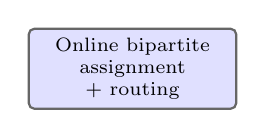
\begin{tikzpicture}
          \node[blk, text width=2.4cm]{Online bipartite\\ assignment + routing};
        \end{tikzpicture}
      \end{block}
    \end{column}
    \begin{column}{0.32\textwidth}
      \begin{block}{Track B — Open Innovation}
        \textbf{CityPulse}\\
        Live Civic Health Dashboard
        \vspace{2mm}
        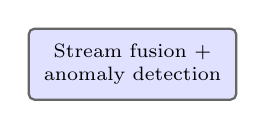
\begin{tikzpicture}
          \node[blk, text width=2.4cm]{Stream fusion +\\ anomaly detection};
        \end{tikzpicture}
      \end{block}
    \end{column}
    \begin{column}{0.32\textwidth}
      \begin{block}{Track C — Deep-Tech}
        \textbf{SentinelAPI}\\
        Zero-Trust API Scanner
        \vspace{2mm}
        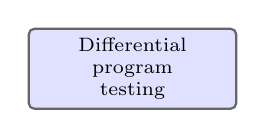
\begin{tikzpicture}
          \node[blk, text width=2.4cm]{Differential program\\ testing};
        \end{tikzpicture}
      \end{block}
    \end{column}
  \end{columns}
\end{frame}

% ================= TRACK A =================
\section{Track A — Surplus-to-Shelter}

\begin{frame}{Track A — Problem Framing}
  \textbf{Not a CRUD app} — an \alert{online bipartite assignment} problem over a
  spatio-temporal stream:
  \begin{itemize}
    \item Donations arrive dynamically:
      $(location, food\_type, qty, expiry, cold\_chain)$
    \item Shelters = resources with capacity \& compatibility constraints
    \item Every donation has a \alert{hard deadline} (expiry) $\Rightarrow$
      deadline-constrained assignment with travel cost
  \end{itemize}

  \begin{block}{Objective}
    Minimize wasted food: match each donation to a compatible shelter that can
    receive it before expiry, at minimum road-network cost.
  \end{block}
\end{frame}

\begin{frame}{Track A — Flow}
  \begin{center}
  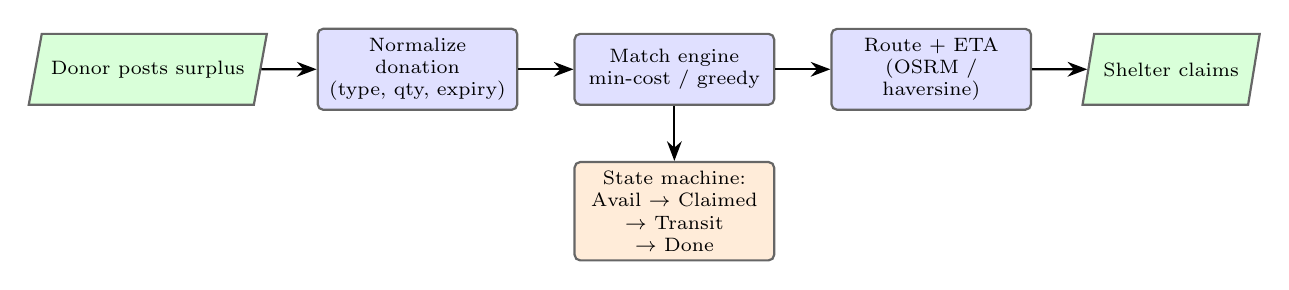
\begin{tikzpicture}[node distance=0.7cm and 0.7cm]
    \node[io] (donor) {Donor posts surplus};
    \node[blk, right=of donor] (feat) {Normalize donation\\(type, qty, expiry)};
    \node[blk, right=of feat] (match) {Match engine\\min-cost / greedy};
    \node[blk, right=of match] (route) {Route + ETA\\(OSRM / haversine)};
    \node[io, right=of route] (shelter) {Shelter claims};
    \node[blk, below=of match, fill=orange!15] (state) {State machine:\\Avail $\to$ Claimed $\to$ Transit $\to$ Done};
    \draw[arr] (donor) -- (feat);
    \draw[arr] (feat) -- (match);
    \draw[arr] (match) -- (route);
    \draw[arr] (route) -- (shelter);
    \draw[arr] (match) -- (state);
  \end{tikzpicture}
  \end{center}
\end{frame}

\begin{frame}[fragile]{Track A — Matching Code}
\begin{lstlisting}[language=Python]
import numpy as np
from scipy.optimize import linear_sum_assignment

def match(donors, shelters):
    n, m = len(donors), len(shelters)
    cost = np.full((n, m), np.inf)          # inf = incompatible
    for i, d in enumerate(donors):
        for j, s in enumerate(shelters):
            if compatible(d, s):            # type + cold-chain + capacity
                cost[i, j] = road_distance(d, s)
    rows, cols = linear_sum_assignment(cost)   # O(n^3) min-cost
    return [(donors[i], shelters[c]) for i, c in zip(rows, cols)
            if cost[i, c] < np.inf]
\end{lstlisting}
\footnotesize MVP: greedy + deadline heap. Ceiling: OR-Tools CP-SAT (routing + assignment).
\end{frame}

\begin{frame}{Track A — Stack \& Steps}
  \begin{columns}[T]
    \begin{column}{0.48\textwidth}
      \textbf{Tech stack}
      \begin{itemize}\small
        \item Backend: \texttt{FastAPI} (async)
        \item Matching: SciPy $\to$ OR-Tools
        \item Roads: haversine $\to$ OSRM
        \item DB: SQLite $\to$ PostGIS
        \item Realtime: WebSocket / SSE
        \item UI: Next.js + MapLibre GL
      \end{itemize}
    \end{column}
    \begin{column}{0.48\textwidth}
      \textbf{Build steps}
      \begin{enumerate}\small
        \item Donation + shelter models
        \item Compatibility \& distance fns
        \item Min-cost matcher
        \item State machine + WebSocket
        \item Live map UI
        \item Demo: post $\to$ match $\to$ ETA
      \end{enumerate}
    \end{column}
  \end{columns}
\end{frame}

% ================= TRACK B =================
\section{Track B — CityPulse}

\begin{frame}{Track B — Problem Framing}
  \textbf{Stream fusion + online anomaly detection} — not a dashboard problem.
  \begin{itemize}
    \item Feeds differ in \alert{rate} (weather hourly, transit per-minute,
      311 bursty), \alert{format}, and \alert{identity} (no common place\_id)
    \item Canonical event model:
      \begin{center}
        $(\text{event\_type},\, t,\,\text{geohash},\,\text{severity},\,\text{source})$
      \end{center}
    \item Correlation must be \alert{honest}: co-occurrence $\neq$ causation —
      label links as ``possibly related''
  \end{itemize}
\end{frame}

\begin{frame}{Track B — Flow}
  \begin{center}
  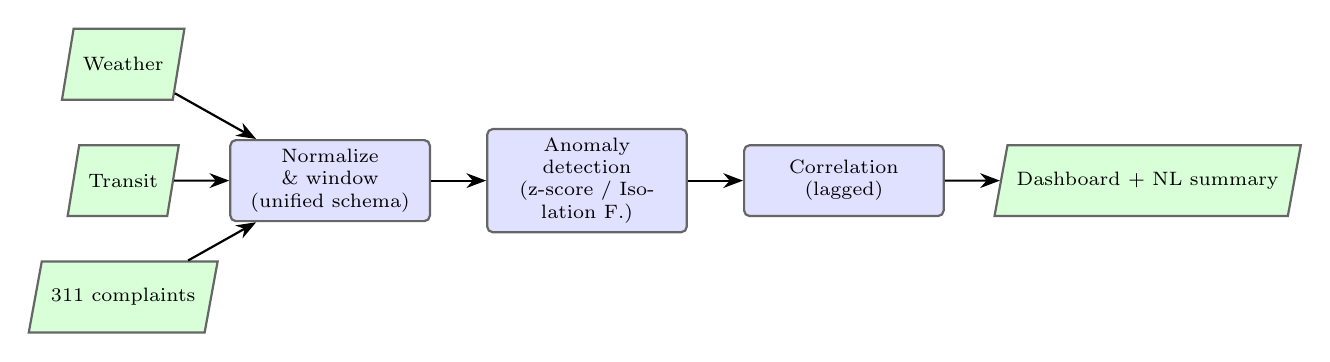
\begin{tikzpicture}[node distance=0.55cm and 0.7cm]
    \node[io] (w) {Weather};
    \node[io, below=of w] (t) {Transit};
    \node[io, below=of t] (c) {311 complaints};
    \node[blk, right=of t] (norm) {Normalize \& window\\(unified schema)};
    \node[blk, right=of norm] (anom) {Anomaly detection\\(z-score / Isolation F.)};
    \node[blk, right=of anom] (corr) {Correlation\\(lagged)};
    \node[io, right=of corr] (dash) {Dashboard + NL summary};
    \draw[arr] (w) -- (norm);
    \draw[arr] (t) -- (norm);
    \draw[arr] (c) -- (norm);
    \draw[arr] (norm) -- (anom);
    \draw[arr] (anom) -- (corr);
    \draw[arr] (corr) -- (dash);
  \end{tikzpicture}
  \end{center}
\end{frame}

\begin{frame}[fragile]{Track B — Anomaly Detection Code}
\begin{lstlisting}[language=Python]
from collections import deque

W = deque(maxlen=1440)                # rolling window

def flag(event):
    W.append(event.value)
    mu = sum(W) / len(W)
    var = sum((x - mu) ** 2 for x in W) / len(W)
    sd = var ** 0.5
    z = (event.value - mu) / (sd + 1e-9)
    return z > 3.0                   # 3-sigma anomaly
\end{lstlisting}
\footnotesize Ceiling: Isolation Forest / STL decomposition / transformer autoencoder.
\end{frame}

\begin{frame}{Track B — Stack \& Steps}
  \begin{columns}[T]
    \begin{column}{0.48\textwidth}
      \textbf{Tech stack}
      \begin{itemize}\small
        \item Ingestion: asyncio pollers $\to$ Kafka/Bytewax
        \item Store: Postgres $\to$ TimescaleDB
        \item Anomaly: z-score $\to$ Isolation Forest
        \item Summary: template NLG $\to$ grounded LLM
        \item UI: Next.js + MapLibre + WebSocket
        \item Replay: seeded synthetic dataset
      \end{itemize}
    \end{column}
    \begin{column}{0.48\textwidth}
      \textbf{Build steps}
      \begin{enumerate}\small
        \item Simulate 3 feeds
        \item Normalize to one schema
        \item Rolling-window anomaly
        \item Lagged correlation
        \item Plain-language summary
        \item Live map + replay
      \end{enumerate}
    \end{column}
  \end{columns}
\end{frame}

% ================= TRACK C =================
\section{Track C — SentinelAPI}

\begin{frame}{Track C — Problem Framing}
  \textbf{Differential program testing} against a spec — not blind fuzzing.
  \begin{itemize}
    \item Compare \alert{behaviour across security contexts} and flag divergence
      from the spec's contract
    \item The oracle = cross-account response diff + schema-vs-actual-keys diff
    \item \alert{Key tactic}: build the sandbox API \emph{and} the scanner, so
      precision is verifiable and the demo is deterministic
  \end{itemize}
  \begin{block}{Classes implemented}
    (1) BOLA / IDOR \quad (2) Excessive data exposure \quad (3)~stretch: broken auth / missing rate-limit
  \end{block}
\end{frame}

\begin{frame}{Track C — Flow}
  \begin{center}
  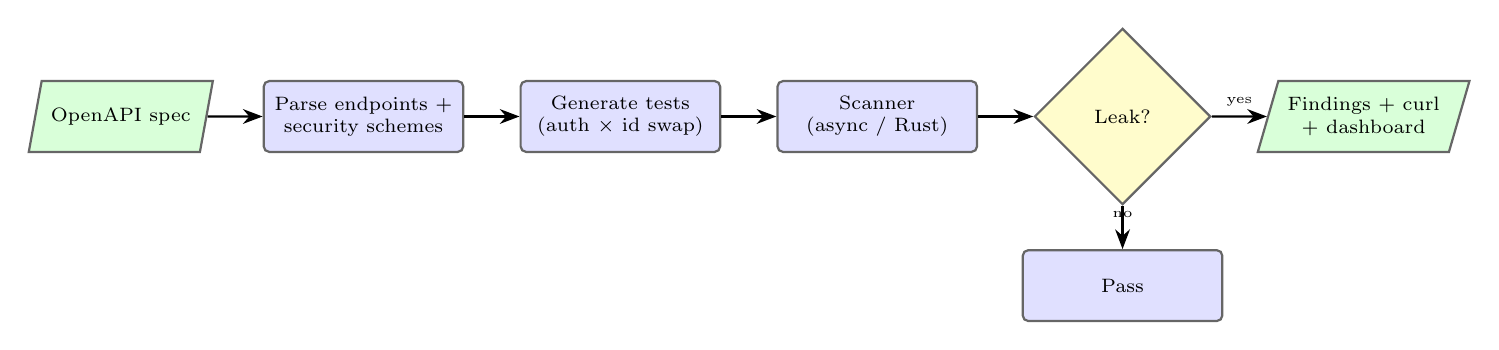
\begin{tikzpicture}[node distance=0.55cm and 0.7cm]
    \node[io] (spec) {OpenAPI spec};
    \node[blk, right=of spec] (parse) {Parse endpoints +\\ security schemes};
    \node[blk, right=of parse] (gen) {Generate tests\\(auth $\times$ id swap)};
    \node[blk, right=of gen] (scan) {Scanner\\(async / Rust)};
    \node[dec, right=of scan, text width=1.6cm] (oracle) {Leak?};
    \node[blk, below=of oracle] (ok) {Pass};
    \node[io, right=of oracle] (find) {Findings + curl\\ + dashboard};
    \draw[arr] (spec) -- (parse);
    \draw[arr] (parse) -- (gen);
    \draw[arr] (gen) -- (scan);
    \draw[arr] (scan) -- (oracle);
    \draw[arr] (oracle) -- node[above, font=\tiny]{no} (ok);
    \draw[arr] (oracle) -- node[above, font=\tiny]{yes} (find);
  \end{tikzpicture}
  \end{center}
\end{frame}

\begin{frame}[fragile]{Track C — IDOR Differential Test}
\begin{lstlisting}[language=Python]
async def test_bola(client, endpoints):
    a, b = await register(client), await register(client)   # two users
    findings = []
    for ep in endpoints_with_id(endpoints):
        r = await client.get(ep.path.format(id=b.id),   # A's token, B's id
                             headers=a.auth)
        if r.json().get("user_id") == b.id:             # cross-account leak
            findings.append(Finding("CRITICAL", "BOLA", ep,
                                    curl_repro(ep, a, b)))
    return findings
\end{lstlisting}
\footnotesize Oracle: response returns a resource owned by a different principal.
\end{frame}

\begin{frame}{Track C — Stack \& Steps}
  \begin{columns}[T]
    \begin{column}{0.48\textwidth}
      \textbf{Tech stack}
      \begin{itemize}\small
        \item Sandbox API: FastAPI (auto OpenAPI)
        \item Engine: Python httpx $\to$ Rust (tokio + reqwest)
        \item Spec: openapi.json / Swagger 2.0
        \item Oracle: schema diff + cross-account diff
        \item Report: findings.json $\to$ dashboard
        \item Advanced: LLM test-gen, agentic chains
      \end{itemize}
    \end{column}
    \begin{column}{0.48\textwidth}
      \textbf{Build steps}
      \begin{enumerate}\small
        \item Seed vulnerable API (IDOR + exposure)
        \item Parse OpenAPI spec
        \item Generate auth-context tests
        \item Differential oracle
        \item Severity ranking + curl repro
        \item Dashboard
      \end{enumerate}
    \end{column}
  \end{columns}
\end{frame}

% ================= COMPARISON =================
\section{Decision}

\begin{frame}{Comparative Summary}
  \centering
  \begin{tabular}{lccc}
    \toprule
    Criterion & A (Food) & B (CityPulse) & C (SentinelAPI) \\
    \midrule
    Time-to-demo & \textbf{Fastest} & Medium & Medium \\
    Finish risk & Low & Medium & Medium \\
    Wow-factor & Medium & High & \textbf{Highest} \\
    External deps & None & 3+ feeds & None \\
    Demo reliability & High & Medium & \textbf{Highest} \\
    Novelty & Medium & Med-High & \textbf{Highest} \\
    \bottomrule
  \end{tabular}

  \vspace{4mm}
  \begin{block}{Recommendation}
    Safest = A. Best wow + still finishable = \alert{C (SentinelAPI)} —
    deterministic demo, zero external dependencies, deep-tech story.
  \end{block}
\end{frame}

\begin{frame}
  \centering
  {\LARGE Thank you}
\end{frame}

\end{document}
